
\documentclass[a4j]{ujarticle}
\usepackage[dvipdfmx]{graphicx}
\usepackage{url} % <--- 就是加了这一行，用来解析参考文献里的网址！

\title{日本におけるデジタル化の状況}
\author{G68442026 张宇航} 
\date{2026年7月6日}

\begin{document}

\maketitle

\section{デジタル競争力ランキング}
国際経営開発研究所(IMD)の調査\cite{imd} によると、日本のデジタル競争力のランキングは図\ref{fig:digital_ranking}に示すように、調査対象の64カ国中、総合で28位、知識分野で25位となっている。
\begin{figure}[htbp]
  \centering
  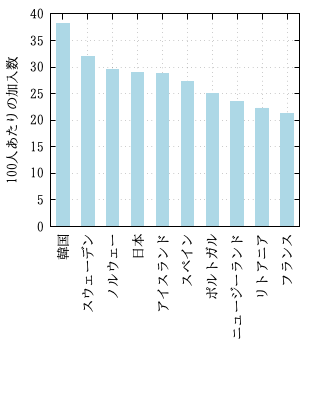
\includegraphics[scale=0.8]{fig11.png}
  \caption{デジタル競争力ランキング（64カ国中）}
  \label{fig:digital_ranking}
\end{figure}

\section{ブロードバンドの整備状況}
OECDによるブロードバンド回線の普及に関する調査\cite{oecd} によると、表\ref{tbl:broadband}に示すように、日本における100人あたりの光ファイバー回線の加入者数は29.0で、韓国、スウェーデン、ノルウェーに続いて第4位になっている。

\begin{table}[htbp]
  \centering
  \caption{光ファイバー回線の加入者数（100人あたり）}
  \label{tbl:broadband}
  \begin{tabular}{|c|l|c|} 
    \hline
    順位 & 国名 & 加入者数 \\
    \hline
    1位 & 韓国 & 38.2 \\
    \hline
    2位 & スウェーデン & 31.9 \\
    \hline
    3位 & ノルウェー & 29.5 \\
    \hline
    4位 & 日本 & 29.0 \\
    \hline
    5位 & アイスランド & 28.8 \\
    \hline
    6位 & スペイン & 27.3 \\
    \hline
    7位 & ポルトガル & 25.1 \\
    \hline
    8位 & ニュージーランド & 23.6 \\
    \hline
    9位 & リトアニア & 22.3 \\
    \hline
    10位 & フランス & 21.2 \\
    \hline
  \end{tabular}
\end{table}

\section{考察}

\begin{itemize}
  \item 日本の光ファイバー回線普及率は世界第4位（29.0人/100人）と高水準にあるが、デジタル競争力の総合順位は28位にとどまっている。このことから、ハードウェアインフラの充実度が、必ずしも国家の総合的なデジタル競争力に直結していないことがわかる。
  \item 特に「知識」分野の順位が25位と低い水準にある。これは、IT人材の不足やデジタル技術の実装能力といったソフト面での課題が原因であると考えられ、社会全体のデジタルトランスフォーメーション（DX）推進が今後の鍵となる。
\end{itemize}

\bibliographystyle{junsrt}
\bibliography{exercise}

\end{document}吧∫